
%(BEGIN_QUESTION)
% Copyright 2006, Tony R. Kuphaldt, released under the Creative Commons Attribution License (v 1.0)
% This means you may do almost anything with this work of mine, so long as you give me proper credit

Et manometer kan brukes til å måle differansetrykk over en innsnevring i et rør. Trykket faller som følge av strømning gjennom røret, noe som gjør at manometeret (indirekte) kan brukes til å måle strømning:

$$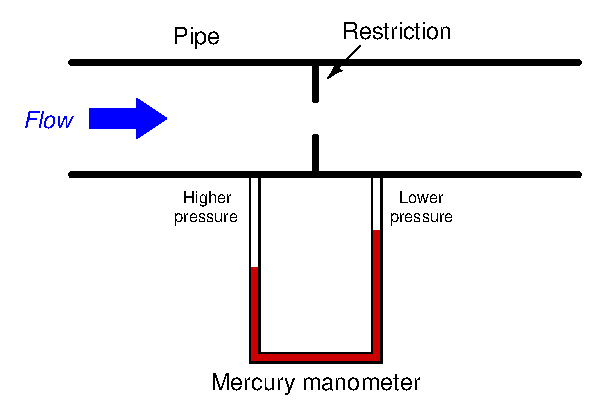
\includegraphics[width=15.5cm]{i00796x01.eps}$$

I eksemplet over er mediet som strømmer i røret luft, og manometeret bruker kvikksølv som indikatorvæske. Hvis vi i stedet prøver å måle volumstrømmen til en {\it væske}, for eksempel vann, med samme metode, vil vi se at manometeret ikke viser helt slik vi kanskje forventer:

$$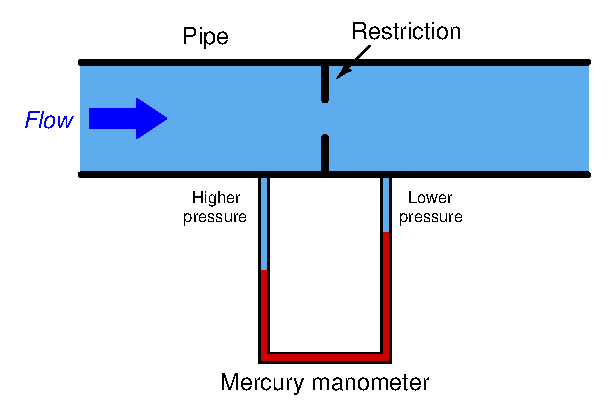
\includegraphics[width=15.5cm]{i00796x02.eps}$$

Det vil si: ved nøyaktig samme differansetrykk fra innsnevringen vil manometeret vise noe annet enn når det måler lufttrykk. Avgjør om manometeret vil vise for høy eller for lav verdi, og forklar {\it hvorfor}.

\underbar{file i00796}
%(END_QUESTION)





%(BEGIN_ANSWER)

Manometeret vil vise for høyt, altså større differansetrykk enn det som faktisk er til stede. Hvis dette er vanskelig å se, kan du tenke deg at væsken i røret hadde nøyaktig samme tetthet som kvikksølvet i manometeret: hva ville {\it det} gjort med kvikksølvet i manometeret ved en gitt $\Delta$P? Sett opp et {\it tankeeksperiment} med bevisst enkle (og ekstreme) forutsetninger, og se etter mønstre du kan generalisere.

\vskip 10pt

Utfordring: utled en matematisk korreksjonsfaktor for å tolke manometeravlesningen til riktig differansetrykk i tommer kvikksølv ($\Delta$P).

%(END_ANSWER)





%(BEGIN_NOTES)

Husk at vannet i manometerrørene (over kvikksølvet) har vekt og danner et ``væskesøyletrykk'' på samme måte som kvikksølvkolonnene!

%INDEX% Measurement, pressure: manometer across an orifice

%(END_NOTES)
